\documentclass{beamer}
\usepackage{ArmenianSlides}

\begin{document}

\title[Decorator]{Նախագծման Ձևանմուշներ։ Decorator}
\author[Հրաչյա Թանդիլյան\copyright]{Հրաչյա Թանդիլյան}
\date{2020}

%-------------------------------------------------------------------------------------------------
\begin{frame}
\titlepage
\end{frame}
%-------------------------------------------------------------------------------------------------

\section{Նպատակը}
%-------------------------------------------------------------------------------------------------
\begin{frame}\frametitle{Decorator}
\begin{block}{Նպատակը}
    Օբյեկտին դինամիկ կերպով հավելյալ պատասխանատվություն է կցում: \\ Հանդիսանում է
    ընդլայնման նպատակով ժառանգման առավել ճկուն այլընտրանք:
\end{block}
\vfill
Նաև հայտնի է որպես
\begin{itemize}
    \item Wrapper
\end{itemize}
\end{frame}
%-------------------------------------------------------------------------------------------------

\subsection{Մոտիվացիան}
%-------------------------------------------------------------------------------------------------
\begin{frame}\frametitle{Մոտիվացիան}
\begin{center}
    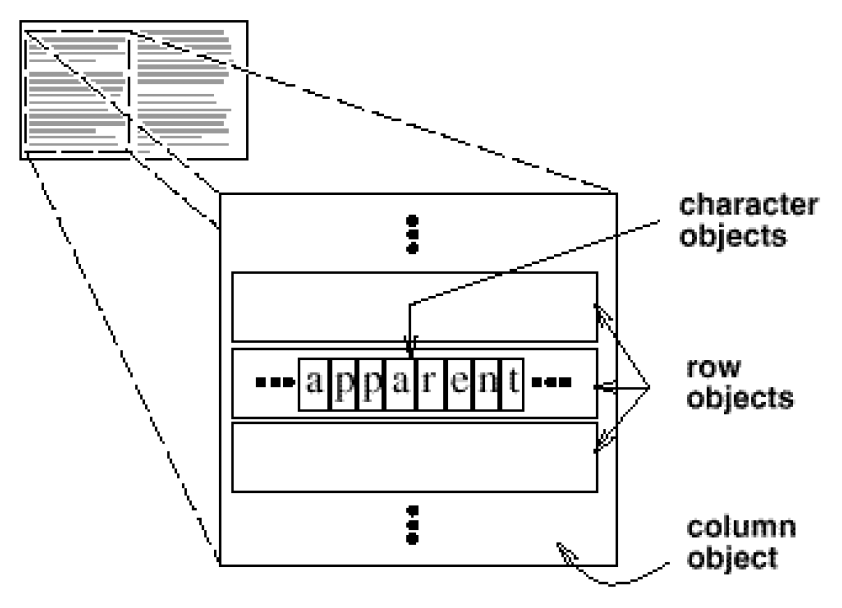
\includegraphics[scale=0.4]{motivation1.png}
    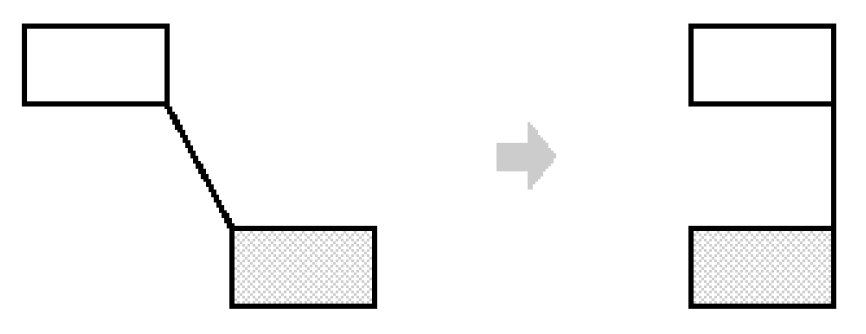
\includegraphics[scale=0.4]{motivation2.png}
\end{center}
\end{frame}
%-------------------------------------------------------------------------------------------------

%-------------------------------------------------------------------------------------------------
\begin{frame}\frametitle{Մոտիվացիան}
\begin{center}
    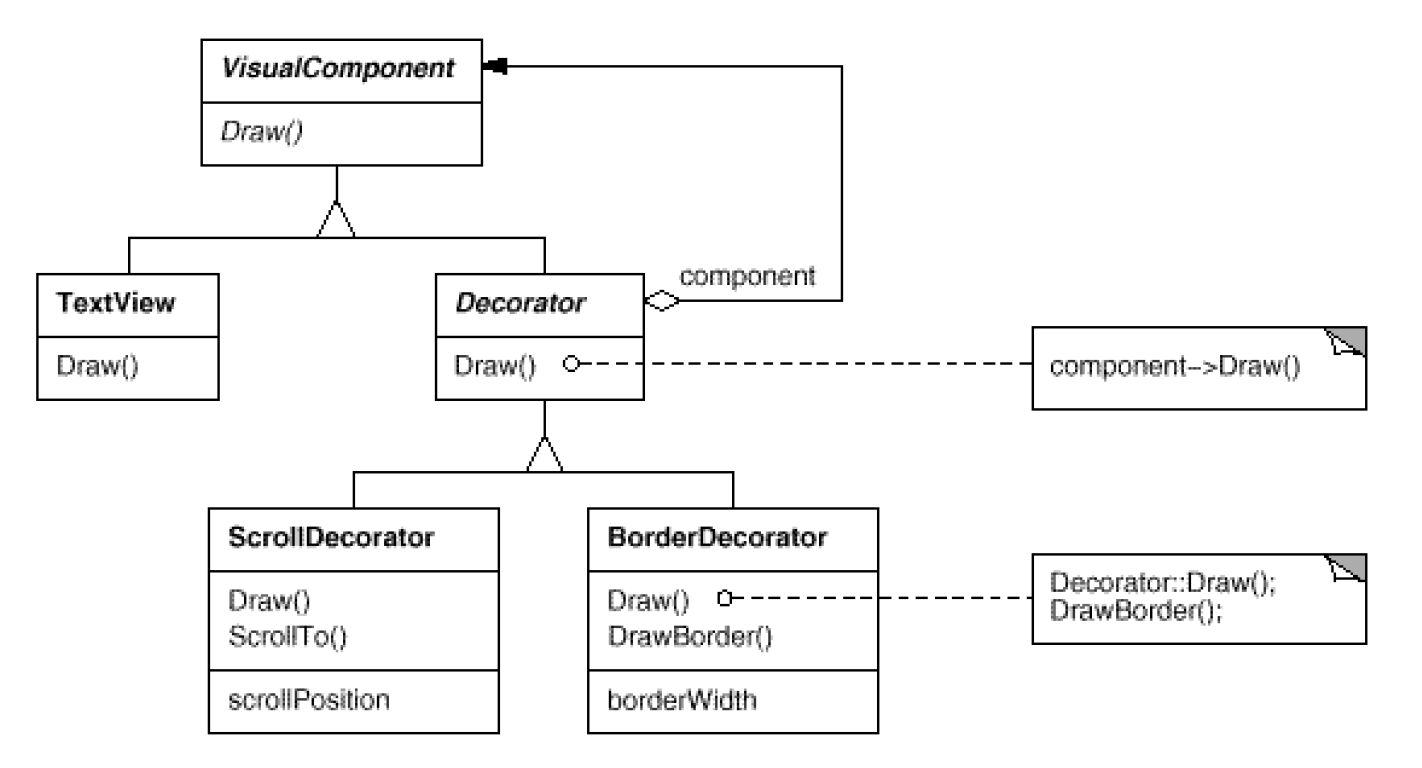
\includegraphics[scale=0.4]{motivation3.png}
\end{center}
\end{frame}
%-------------------------------------------------------------------------------------------------

\subsection{Կիրառելիությունը}
%-------------------------------------------------------------------------------------------------
\begin{frame}\frametitle{Կիրառելիությունը}
Այս Ն.Ձ. պետք է օգտագործել երբ.
\vfill
\scriptsize
\setbeamertemplate{itemize/enumerate subbody begin}{\scriptsize}
\begin{enumerate}
    \item Անհրաժեշտ է անհատական օբյեկտի դինամիկ և թափանցիկ կերպով
    հավելյալ պատասխանատվություն տալ առանց մնացյալ օբյեկտների վրա ազդելու: \vfill
    \item Անհրաժեշտ է օբյեկտի այնպիսի պատասխանատվություն տալ,
    որը հնարավոր լինի չեղարկել: \vfill
    \item Երբ ժառանգման միջոցով ընդլայնումը կիրառելի չէ. \vfill
    \begin{itemize}
        \item Երբ մեծ քանակով անկախ ընդլայնումների կարիք կա, բայց բոլոր կոմբինացիաների
        համար ժառանգ դասերի ստեղծումը կբերի դասերի քանակի չափից ավել աճի: \vfill
        \item Երբ դասի սահմանումը թաքնված է կամ հասանելի չէ ժառանգման համար:
    \end{itemize}
\end{enumerate}
\end{frame}
%-------------------------------------------------------------------------------------------------

\section{Կառուցվածքը}
%-------------------------------------------------------------------------------------------------
\begin{frame}\frametitle{Կառուցվածքը}
\begin{center}
    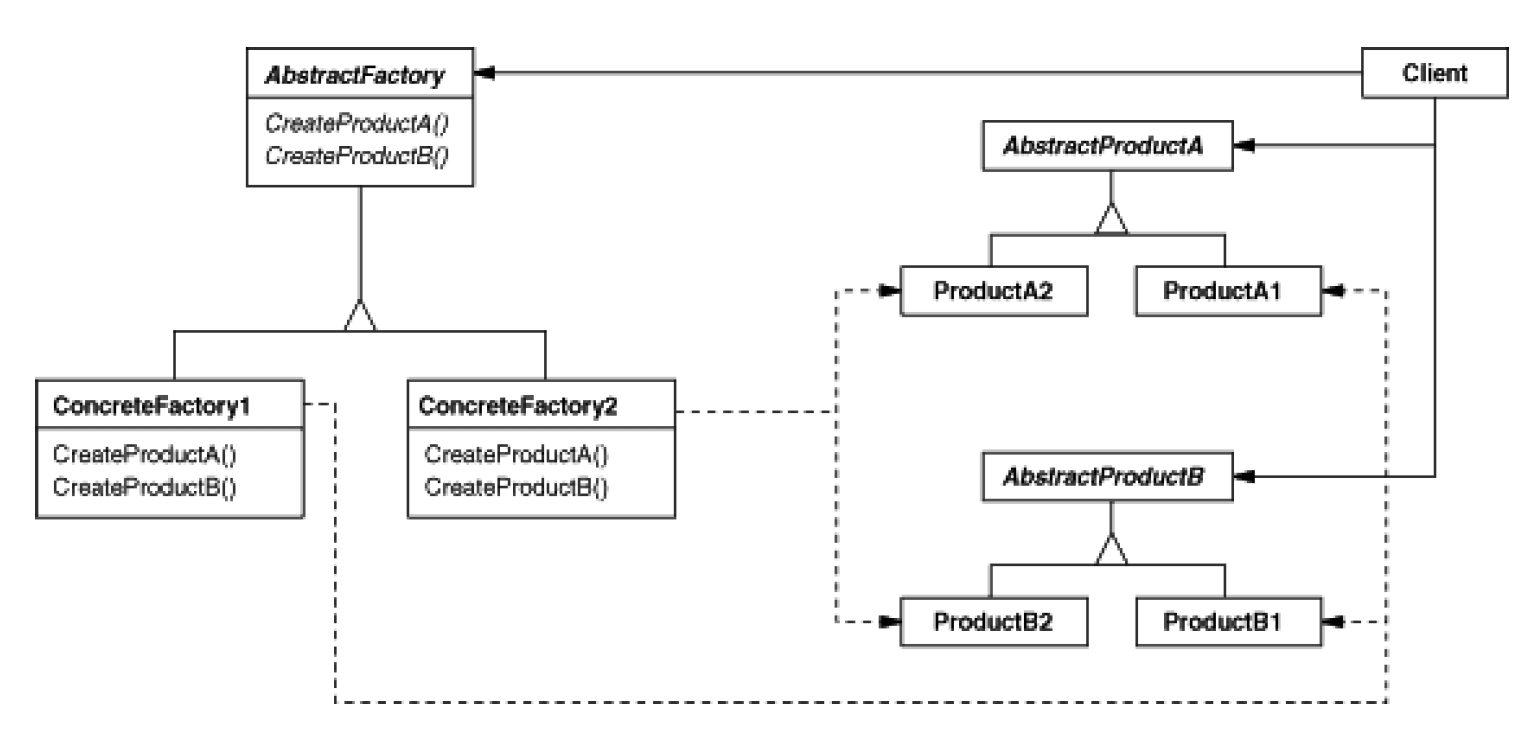
\includegraphics[scale=0.4]{structure.png}
\end{center}
\end{frame}
%-------------------------------------------------------------------------------------------------

\subsection{Հետևանքները}
%-------------------------------------------------------------------------------------------------
\begin{frame}\frametitle{Հետևանքները}
Այս Ն.Ձ. ունի հետևյալ առավելություններն ու թերությունները.
\vfill
\begin{enumerate}
    \item Առավել ճկուն է քան ստատիկ ժառանգումը: \pause \vfill
    \item Խուսափում է հատկություններով հարուստ դասերի հիերարխիայով
    վեր բարձրացումից: \pause \vfill
    \item Դեկորատորը և նրա կոմպոնենտը միևնույն օբյեկտը չեն: \pause \vfill
    \item Բերում է մեծ քանակով փոքր օբյեկտների ստեղծման:
\end{enumerate}
\end{frame}
%-------------------------------------------------------------------------------------------------

\section{Իրականացումը}
%-------------------------------------------------------------------------------------------------
\begin{frame}\frametitle{Իրականացումը}
\begin{enumerate}
    \item Ինտերֆեյսի պահպանում: \vfill
    \item Աբստրակտ դեկորատոր դասի բացակայություն: \vfill
    \item Կոմպոնենտ դասերի պարզ (lightweight) իրականացում: \vfill
    \item Օբյեկտի արտաքինի փոխարինումն ի տարբերություն օբյեկտի ներքինի փոխարինման:
\end{enumerate}
\end{frame}
%-------------------------------------------------------------------------------------------------

\subsection{Օրինակ}
%-------------------------------------------------------------------------------------------------
\begin{frame}\frametitle{Օրինակ}
\begin{center}
    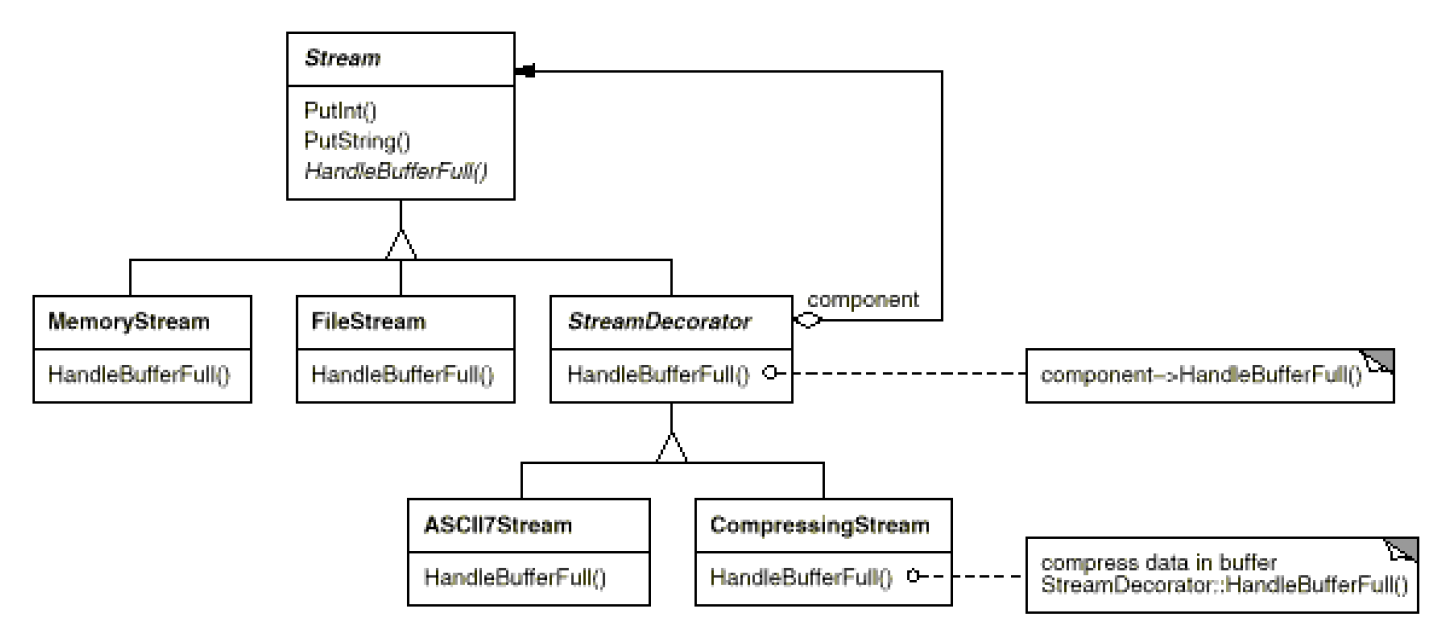
\includegraphics[scale=0.4]{example.png}
\end{center}
\end{frame}
%-------------------------------------------------------------------------------------------------

%-------------------------------------------------------------------------------------------------
\begin{frame}[fragile]\frametitle{Օրինակ}
\begin{english}
\begin{minted}[fontsize=\scriptsize]{cpp}
class VisualComponent {

public:
    VisualComponent();
    virtual void Draw();
    virtual void Resize();
};

class Decorator : public VisualComponent {

public:
    Decorator(VisualComponent*);

    virtual void Draw() { component->Draw(); }
    virtual void Resize() { component->Resize(); }

private:
    VisualComponent* component;
};
\end{minted}
\end{english}
\end{frame}
%-------------------------------------------------------------------------------------------------

%-------------------------------------------------------------------------------------------------
\begin{frame}[fragile]\frametitle{Օրինակ}
\begin{english}
\begin{minted}{cpp}
class BorderDecorator : public Decorator {

public:
    BorderDecorator(VisualComponent*, int borderWidth);

    virtual void Draw() {
        Decorator::Draw();
        DrawBorder(width);
    }

private:
    void DrawBorder(int);
    int width;
};
\end{minted}
\end{english}
\end{frame}
%-------------------------------------------------------------------------------------------------

%-------------------------------------------------------------------------------------------------
\begin{frame}[fragile]\frametitle{Օրինակ}
\begin{english}
\begin{minted}{cpp}
Window* window = new Window;

TextView* textView = new TextView;

window->SetContents( new BorderDecorator(
                        new ScrollDecorator( textView ), 1) );
\end{minted}
\end{english}
\end{frame}
%-------------------------------------------------------------------------------------------------

\section{Առնչվող Ձևանմուշները}
%-------------------------------------------------------------------------------------------------
\begin{frame}\frametitle{Առնչվող Նախագծման Ձևանմուշները}
\begin{itemize}
    \item Adapter \vfill
    \item Composite \vfill
    \item Strategy
\end{itemize}
\end{frame}
%-------------------------------------------------------------------------------------------------

\end{document}
